\documentclass[letterpaper, 10 pt, conference]{ieeeconf}  % Comment this line out
                                                          % if you need a4paper
%\documentclass[a4paper, 10pt, conference]{ieeeconf}      % Use this line for a4
                                                          % paper

\IEEEoverridecommandlockouts                              % This command is only
                                                          % needed if you want to
                                                          % use the \thanks command
\overrideIEEEmargins
% See the \addtolength command later in the file to balance the column lengths
% on the last page of the document



% The following packages can be found on http:\\www.ctan.org
%\usepackage{graphics} % for pdf, bitmapped graphics files
%\usepackage{epsfig} % for postscript graphics files
%\usepackage{mathptmx} % assumes new font selection scheme installed
%\usepackage{times} % assumes new font selection scheme installed
%\usepackage{amsmath} % assumes amsmath package installed
%\usepackage{amssymb}  % assumes amsmath package installed

\usepackage{graphicx}


\title{\LARGE \bf
Passively Finding Distance Between an Access Point \& a Mobile Device
}

%\author{ \parbox{3 in}{\centering Huibert Kwakernaak*
%         \thanks{*Use the $\backslash$thanks command to put information here}\\
%         Faculty of Electrical Engineering, Mathematics and Computer Science\\
%         University of Twente\\
%         7500 AE Enschede, The Netherlands\\
%         {\tt\small h.kwakernaak@autsubmit.com}}
%         \hspace*{ 0.5 in}
%         \parbox{3 in}{ \centering Pradeep Misra**
%         \thanks{**The footnote marks may be inserted manually}\\
%        Department of Electrical Engineering \\
%         Wright State University\\
%         Dayton, OH 45435, USA\\
%         {\tt\small pmisra@cs.wright.edu}}
%}

\author{Muhammad Yasoob Ullah Khalid$^{1}$ and Aaron Gember-Jacobson$^{2}$% <-this % stops a space
\thanks{$^{1}$Muhammad Yasoob Ullah Khalid is a Sophomore at Colgate University, Hamilton, NY 13346, USA
        {\tt\small ykhalid at colgate.edu}}%
\thanks{$^{2}$Aaron Gember-Jacobson is with the Department of Computer Science, Colgate University, Hamilton, NY 13346, USA
        {\tt\small agemberjacobson at colgate.edu}}%
}


\begin{document}



\maketitle
\thispagestyle{empty}
\pagestyle{empty}


%%%%%%%%%%%%%%%%%%%%%%%%%%%%%%%%%%%%%%%%%%%%%%%%%%%%%%%%%%%%%%%%%%%%%%%%%%%%%%%%
\begin{abstract}

Will be filled at the very end

\end{abstract}


%%%%%%%%%%%%%%%%%%%%%%%%%%%%%%%%%%%%%%%%%%%%%%%%%%%%%%%%%%%%%%%%%%%%%%%%%%%%%%%%
\section{INTRODUCTION}

According to the Uniform Crime Report 90,185 rape cases were filed with the police in US in 2015. This is just the count of those cases which were filed, there are tons of other cases which people did not even bother filing. A big reason for unfiled cases is that a lot of these rapes/sexual assaults happen when the victim is under the influence of Alcohol/drugs so he/she is not able to remember or identify who the culprit is. There has been a lot of research in this field but nothing concrete has yet come out of it. I believe that with the advancement in technology there must be a way to fight this problem. 

\section{LITERATURE REVIEW}

\subsection{Using ack/res cycle of unicast data packets}

In this method, we have control of one device which is connected to the other one. Let’s assume that we have access to the mobile device and we are connected to the router. IEEE 802.11 specification states that if a device receives a data packet it needs to send an immediate acknowledgement to the sender. The time spent at the receiving end to process the packet and sending an acknowledgement is highly predictable and this MAC processing time is standardized according to IEEE 802.11. This processing time is known as Short Interframe Space (SIFS) and might vary slightly from one device to another due to different WLAN chipsets. 
The basic formulae for calculating the distance between the two devices is:

$$distance =  c.\frac{T_{end}- T_{start} - SIFS}{2}$$
$$where\ c \approx 3.10^8\ m/s\ being\ the\ speed\ of\ light$$

There are multiple issues which need to be catered to while using this method. The first one is the clock timing. An timing error of 1 µs can lead to a distance error of 300 m so it is extremely necessary to use precise clocks. We can make use of the PHY layer and measure the timing on the WLAN card hardware layer.

The reason this method can’t be used in our case is that this method requires access to at least one device. We want our system to be passive and non-intrusive so we can not demand access to any device. We are essentially trying to figure out a way where a similar method can be employed and we can measure the timing as a third party.


\subsection{Location Estimation using MAC address and WiGLE}

This is a really simple method. You intercept the wireless communication between the mobile and the AP using a 3rd device. You record the MAC address and the SSID of the AP and query it against the WiGLE database. WiGLE contains around 349 Million+ APs in its database and there is a high probability that the AP in your proximity is also listed there. This way you will get a probable location of the mobile device with a huge error rate. We can estimate the distance based on how powerful the router is and how much area it covers.

\begin{center}
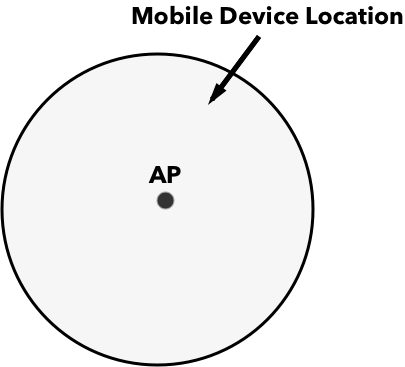
\includegraphics[width=6cm]{Slice_1.png}
\end{center}

This method does not work in our case because we want more fine-grained information. We are aiming for an error rate of around 1 m at max which is not possible by this method. 

\subsection{Localizing using RSSI from Multiple Access Points}

In this method we have access to multiple access points spread throughout an area. The target mobile device is in the range of at least 4-5 Access Points. We try to triangulate the location of the target mobile device using the RSSI value on these access points. We know the exact location of the APs so it is only a matter of some mathematical calculations before we get the exact location of the target mobile. The more access points we have access to, the more accurate the detected location of the target mobile device.

\begin{center}
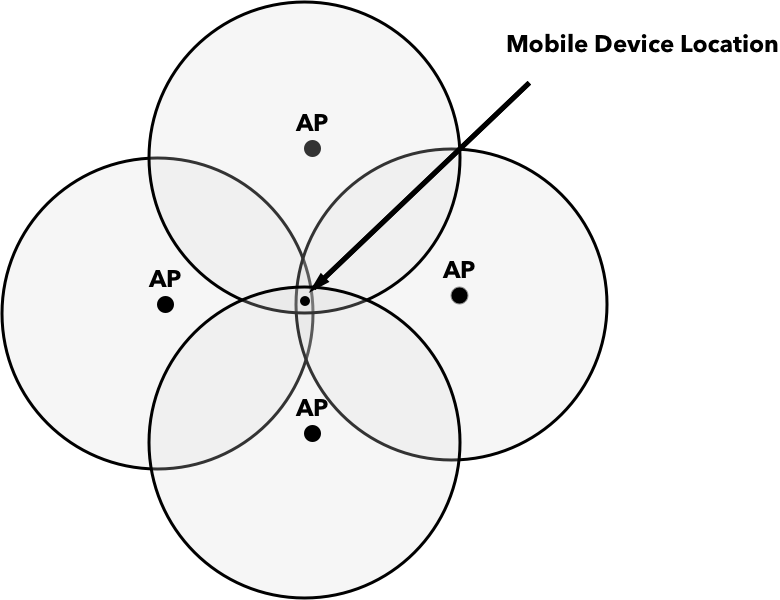
\includegraphics[width=6cm]{Slice_2.png}
\end{center}

This method does not work for us because we don’t have access to so many Access Points. In our ideal scenario we will have no physical access to any Access Point. 

\subsection{ToF measurement by emulating UWB radio}

In this research paper, researchers try to emulate an UWB (Ultra Wideband) radio using off-the-shelf WiFi cards. Each WiFi frequency band is only tens of Megahertz wide but when you join multiple such bands together, you get a very wide bandwidth. Their tool (Chronos) transmits packets on multiple WiFi bands and stitches their information together to give the illusion of an UWB radio. 
By multiplying ToF with the speed of light, AP computes distance between its antennas and the client, hence localizing it. Time resolution is inversely related to the radio bandwidth so more precise readings are possible with an UWB radio.

We can not use this method because it requires access to both devices and requires the Intel 5300 WiFi card to be installed on both devices. 


\section{CURRENT SITUATION}

\subsection{Research Question} 

Can we find the distance between a mobile device and a router without having physical access to both?

\subsection{Ideal Solution}

Our ideal solution involves having three devices. One is going to be the access point, second is going to be the target mobile device and the third device is going to be our own mobile phone. We will not have physical access to the target mobile. The only common thing between these devices will be that our own mobile and the target mobile will be connected to the same AP. 
We will send data packets to the AP and calculate the distance between our device and the AP based on ToF measurements. We will then try to send unsolicited control packets to the target mobile from our device and try to use ToF again to calculate the distance between our device and the target mobile. When we get both of these measurements we can use geometry to figure out the distance between the target mobile device and the router.

\begin{center}
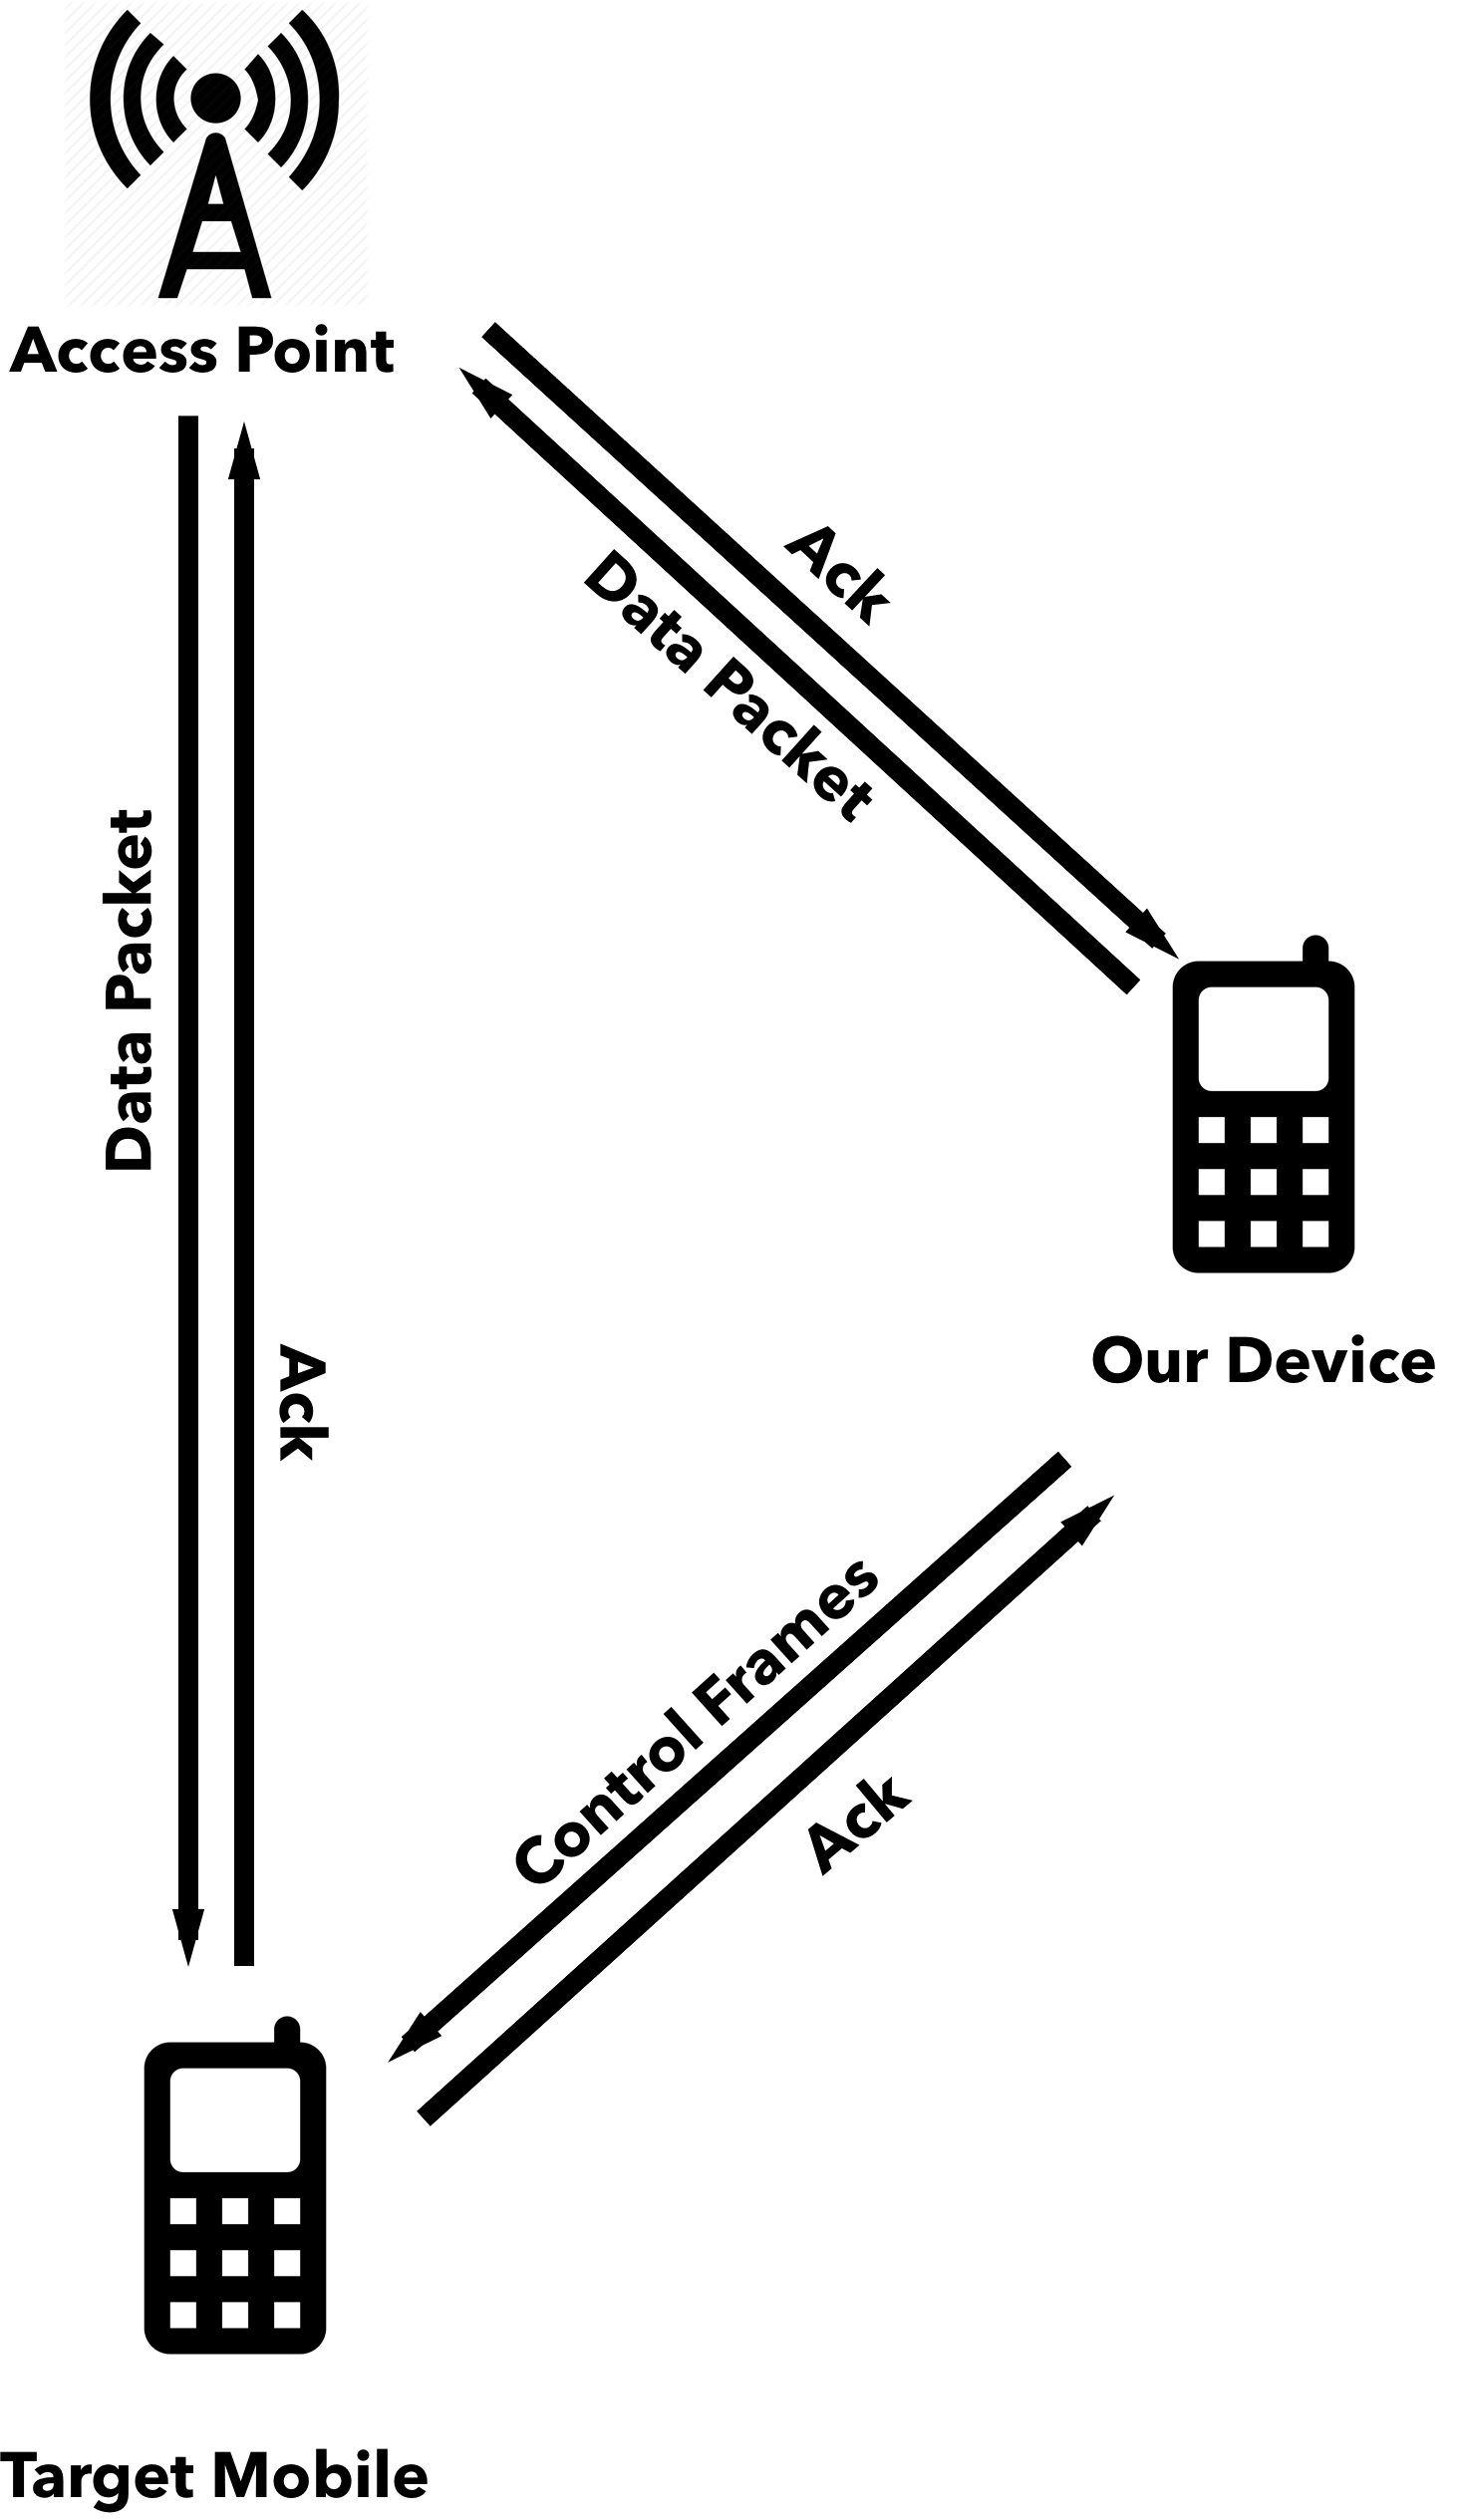
\includegraphics[width=6cm]{Slice_3.png}
\end{center}

\subsection{Current Issues}

We don’t know whether we can force a mobile to send a response to unwanted control packets from our device. Even if that is possible we don’t know whether the time taken by the target mobile to respond is predictable or not. In normal situations when you send a data packet the target mobile has to send an ack within a fixed time but if we are sending unwanted “control” packets, will the mobile respond within a fixed time?

\section*{APPENDIX}

Appendixes should appear before the acknowledgment.

\section*{ACKNOWLEDGMENT}

The preferred spelling of the word ÒacknowledgmentÓ in America is without an ÒeÓ after the ÒgÓ. Avoid the stilted expression, ÒOne of us (R. B. G.) thanks . . .Ó  Instead, try ÒR. B. G. thanksÓ. Put sponsor acknowledgments in the unnumbered footnote on the first page.

References are important to the reader; therefore, each citation must be complete and correct. If at all possible, references should be commonly available publications.



\begin{thebibliography}{99}

%This bibliography will soon be replaced


\bibitem{c1} G. O. Young, ÒSynthetic structure of industrial plastics (Book style with paper title and editor),Ó 	in Plastics, 2nd ed. vol. 3, J. Peters, Ed.  New York: McGraw-Hill, 1964, pp. 15Ð64.
\bibitem{c2} W.-K. Chen, Linear Networks and Systems (Book style).	Belmont, CA: Wadsworth, 1993, pp. 123Ð135.
\bibitem{c3} H. Poor, An Introduction to Signal Detection and Estimation.   New York: Springer-Verlag, 1985, ch. 4.
\bibitem{c4} B. Smith, ÒAn approach to graphs of linear forms (Unpublished work style),Ó unpublished.
\bibitem{c5} E. H. Miller, ÒA note on reflector arrays (Periodical styleÑAccepted for publication),Ó IEEE Trans. Antennas Propagat., to be publised.
\bibitem{c6} J. Wang, ÒFundamentals of erbium-doped fiber amplifiers arrays (Periodical styleÑSubmitted for publication),Ó IEEE J. Quantum Electron., submitted for publication.
\bibitem{c7} C. J. Kaufman, Rocky Mountain Research Lab., Boulder, CO, private communication, May 1995.
\bibitem{c8} Y. Yorozu, M. Hirano, K. Oka, and Y. Tagawa, ÒElectron spectroscopy studies on magneto-optical media and plastic substrate interfaces(Translation Journals style),Ó IEEE Transl. J. Magn.Jpn., vol. 2, Aug. 1987, pp. 740Ð741 [Dig. 9th Annu. Conf. Magnetics Japan, 1982, p. 301].
\bibitem{c9} M. Young, The Techincal Writers Handbook.  Mill Valley, CA: University Science, 1989.


\end{thebibliography}
\end{document}